%\section{Results} 

The total uncertainties on the measured cross sections are 20-25\% with comparable 
contributions from statistical and systematic uncertainties. The largest systematic uncertainty 
is due to the integrated flux uncertainty at 10\%. A detailed discussion of the flux systematic 
uncertainty is presented in Ref.~\cite{nubarprl}. The next largest contribution to the 
systematic uncertainty is the 8\% normalization uncertainty from the background fit. 
The other smaller contributions include the neutrino cross-section models, FSI models, 
and detector simulation systematics. These systematic uncertainties enter the measured 
cross sections through background subtraction, detector resolution, and efficiency corrections. 
The neutrino cross-section model and FSI model uncertainties are evaluated by GENIE. 
The systematic uncertainties on the estimated background is small since the background rate is constrained by data. 
%evaluated by event re-weighting in GENIE. 
Systematic errors in the detector response must be independently estimated.
The uncertainty in neutron response is evaluated by changing the neutron inelastic 
cross section within experimental uncertainties~\cite{Abfalterer:2001gw,Schimmerling:1973bb,
Voss:1956,Slypen:1995fm,Franz:1989cf,Tippawan:2008xk,Bevilacqua:2013rfq,Zanelli:1981zz}
through event reweighting. The reweighting is applied to the leading neutron in the event. 
A large fraction of the secondary $\pi^0$ in the background is estimated to arise from $\pi^{-} \rightarrow \pi^0$
CEX, for which the cross sections are poorly known. The effect of this uncertainty on our 
measurement is evaluated by changing the CEX cross section within its 
uncertainty of $\pm$50\%~\cite{Ashery:1981tq,Bowles:1981,Jones:1993}, and then 
re-measuring the cross sections. Finally, the electromagnetic energy scale uncertainty (2.2\%) 
is taken from the fitted mean uncertainty of the data $m_{\gamma\gamma}$ distribution. 
Flux-integrated single differential cross sections in $\pi^0$ momentum and angle with 
statistical, systematic, and total uncertainties are summarized in 
Tables.\footnoteremember{footsupp1}{See Supplemental Material\ \SuppLocation}


\section{Results and discussion}

The measured differential cross sections as function of $\pi^0$ 
momentum and angle with respect to the beam direction are shown in 
Figures.~\ref{fig:xsec-pimom} and \ref{fig:xsec-pitheta}, respectively. 
The data are compared to the predictions from GENIE with and without FSI.
Above $\unit[0.7]{GeV/c}$, FSI effects have little influence on the 
$\pi^0$ momentum distribution, and both predictions are in good agreement 
with the data.  For momenta below $\unit[0.3]{GeV/c}$, 
inclusion of FSI gives an increased and shifted cross section relative to the no FSI case.
This trend is exhibited by the data; GENIE calculations with and without 
FSI give a $\chi^2$ of $25.4$ and $50.0$ for 11 degrees of freedom (dof), respectively.  
For the distribution of $\pi^0$ production angle in Fig.~\ref{fig:xsec-pitheta}, 
inclusion of FSI into the GENIE simulation results in a mild flattening of the 
distribution with no significant improvement in the $\chi^2$ compared to the 
no FSI case, 16.7 versus 16.0 for 11 degrees of freedom.  Thus the effects of FSI are more pronounced with respect to 
$\pi^0$ momenta than with $\pi^0$ production angle.  This situation likely reflects 
the influence of the $\Delta(1232)$ resonance, which gives a particularly strong 
momentum dependence to the pion-nucleus interaction for 
$p_\pi \approx 0.26$ GeV/c where the pion-carbon cross section is maximum.

\begin{figure}[t]
%\begin{figure}[!htpb]
\centering
\ifnum\PLsupp=0
  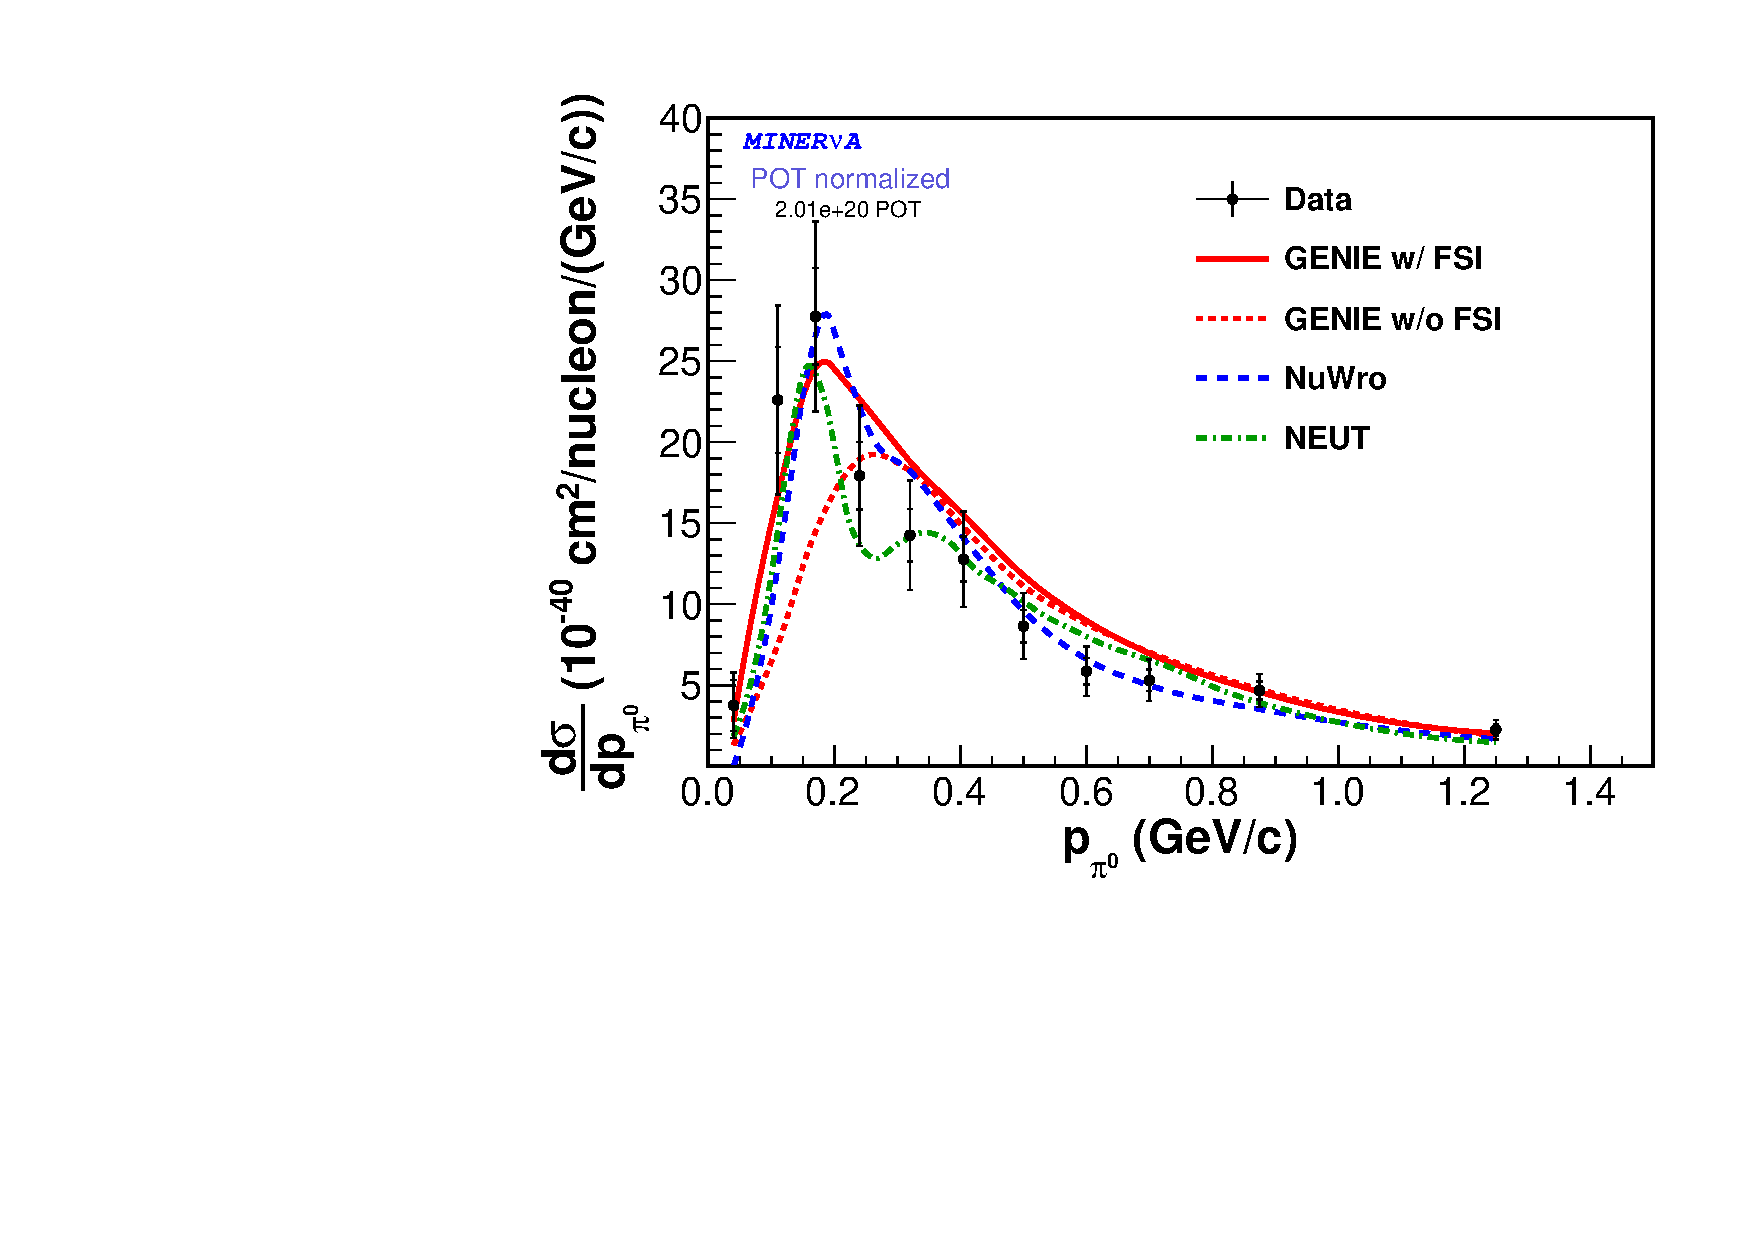
\includegraphics[width=1.0\columnwidth]{pimom-data-mc-xs-multiflux-model-nuwro-pot.pdf}
\else
  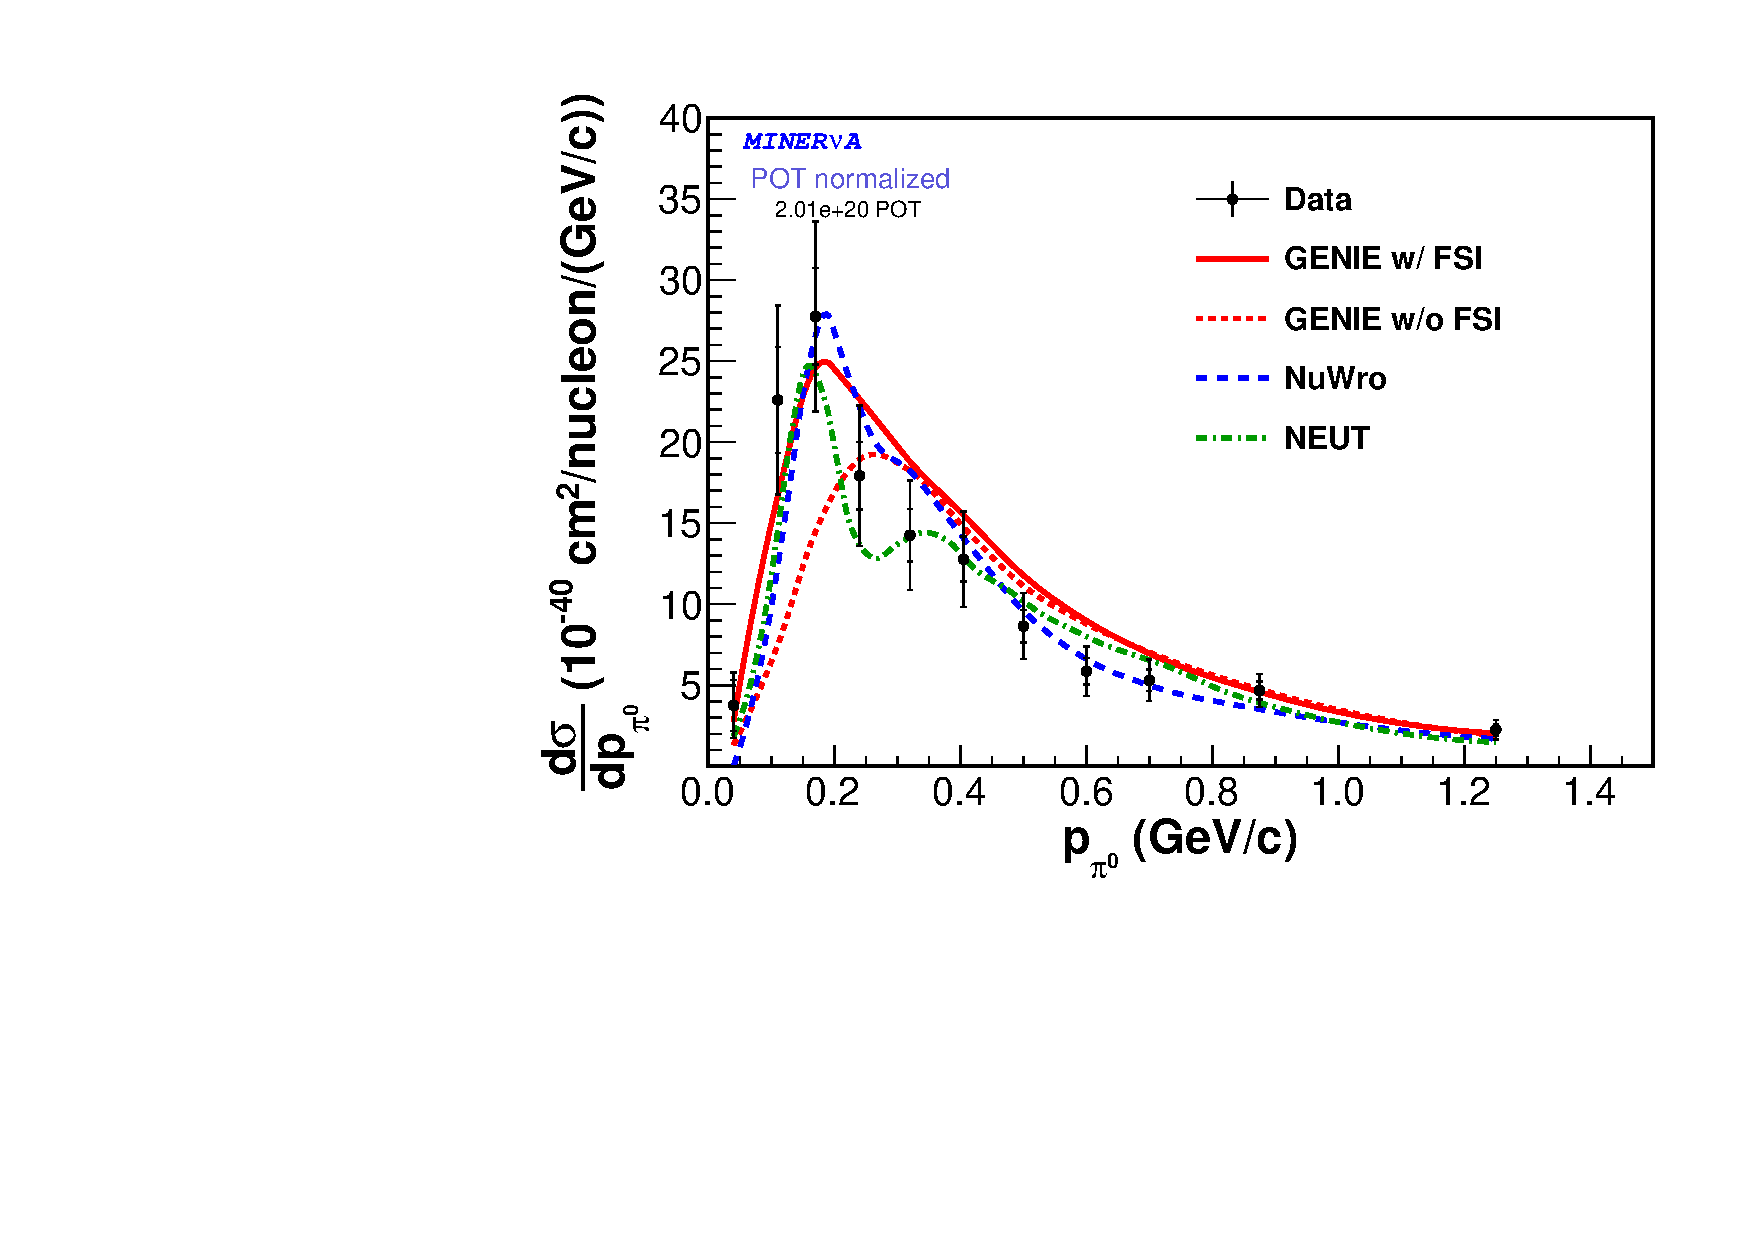
\includegraphics[width=1.0\columnwidth]{pimom-data-mc-xs-multiflux-model-nuwro-pot.pdf}
\fi
\vspace{-7pt}
\caption{Differential cross section for $1\pi^0$ production as function of $\pi^0$ momentum. 
Data are shown as solid circles. 
The inner (outer) error bars correspond to statistical (total) uncertainties. 
The solid (dashed) histograms are 
GENIE prediction with (without) FSI, the long-dashed histogram is the prediction from the NuWro generator, 
and the dot-dashed histogram is the prediction from NEUT.}

\label{fig:xsec-pimom}
\end{figure}


\begin{figure}[!ht]
%\begin{figure}[!htpb]
\centering
\ifnum\PLsupp=0
  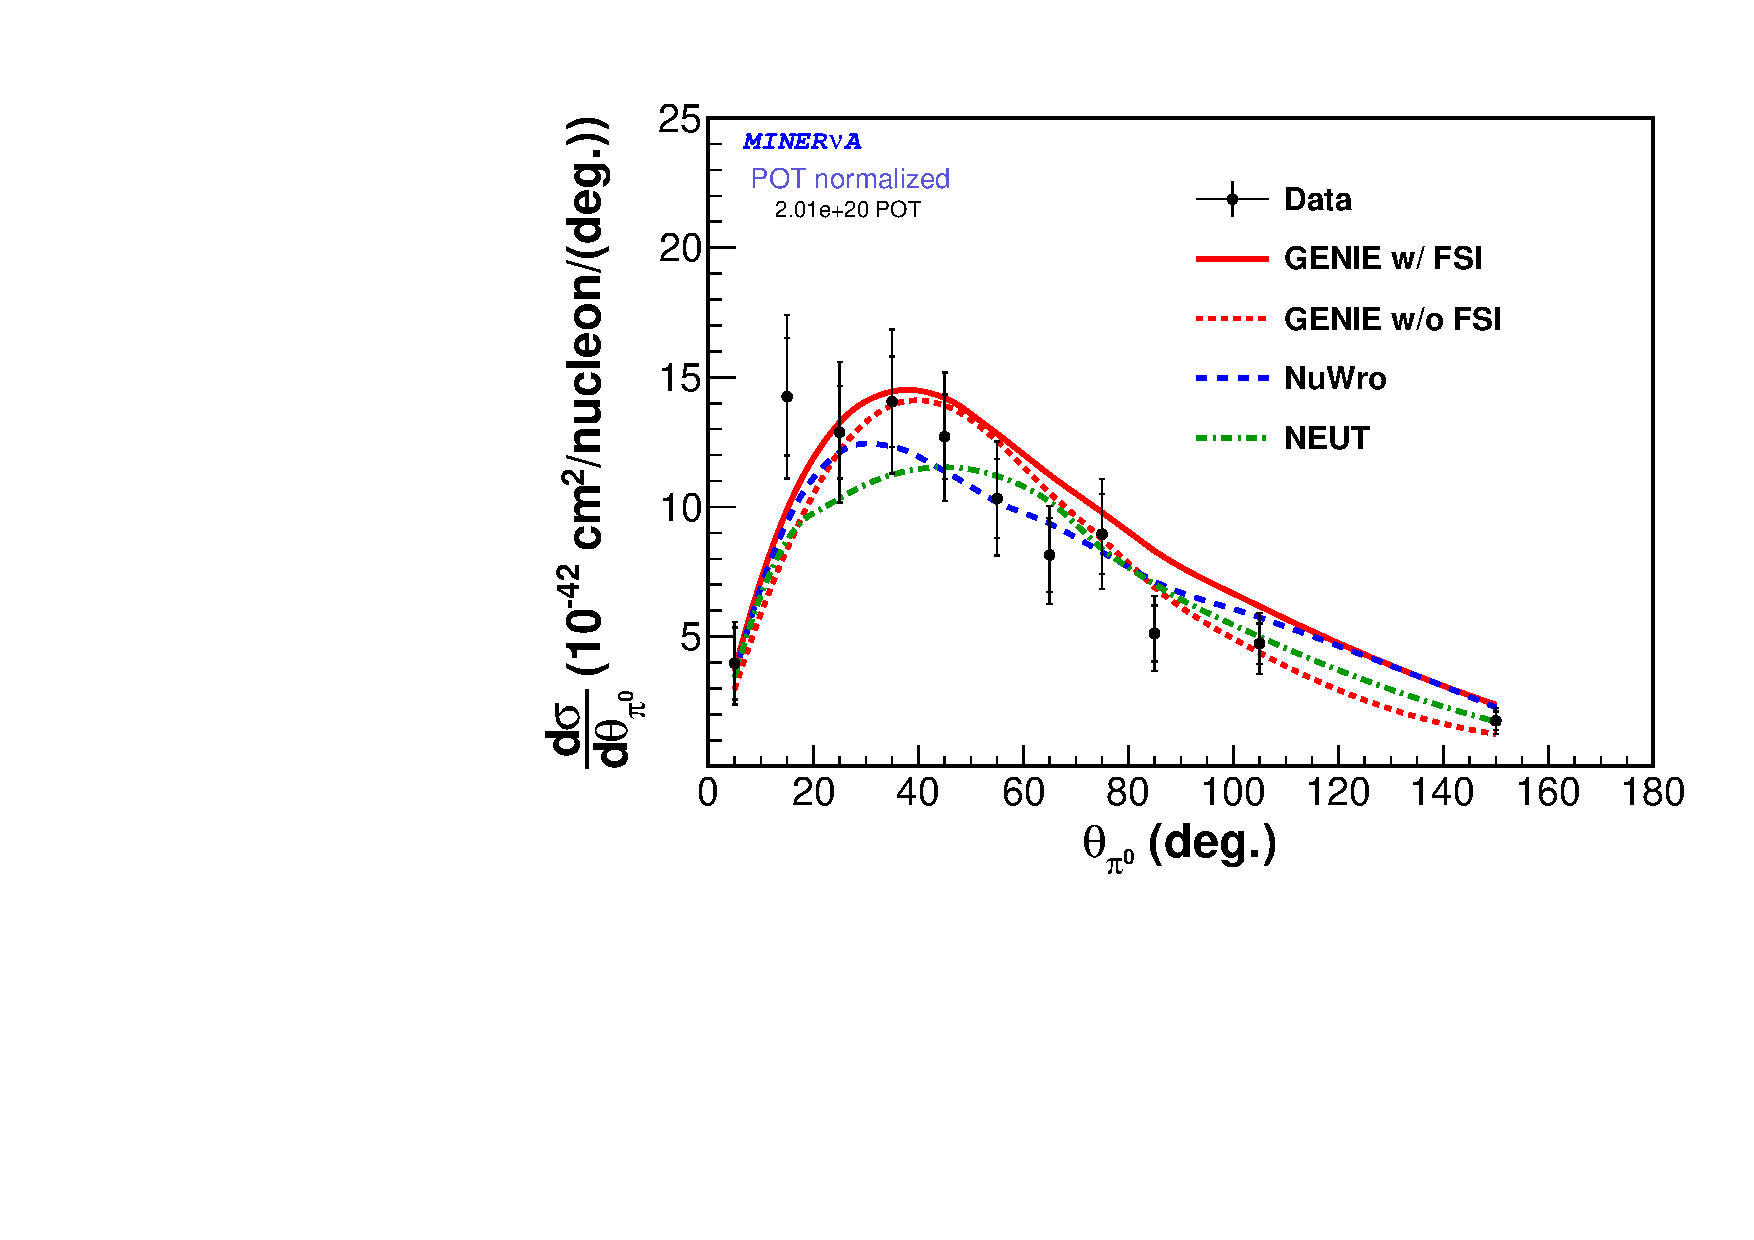
\includegraphics[width=1.0\columnwidth]{theta-data-mc-xs-multiflux-model-nuwro-pot.pdf}
\else
  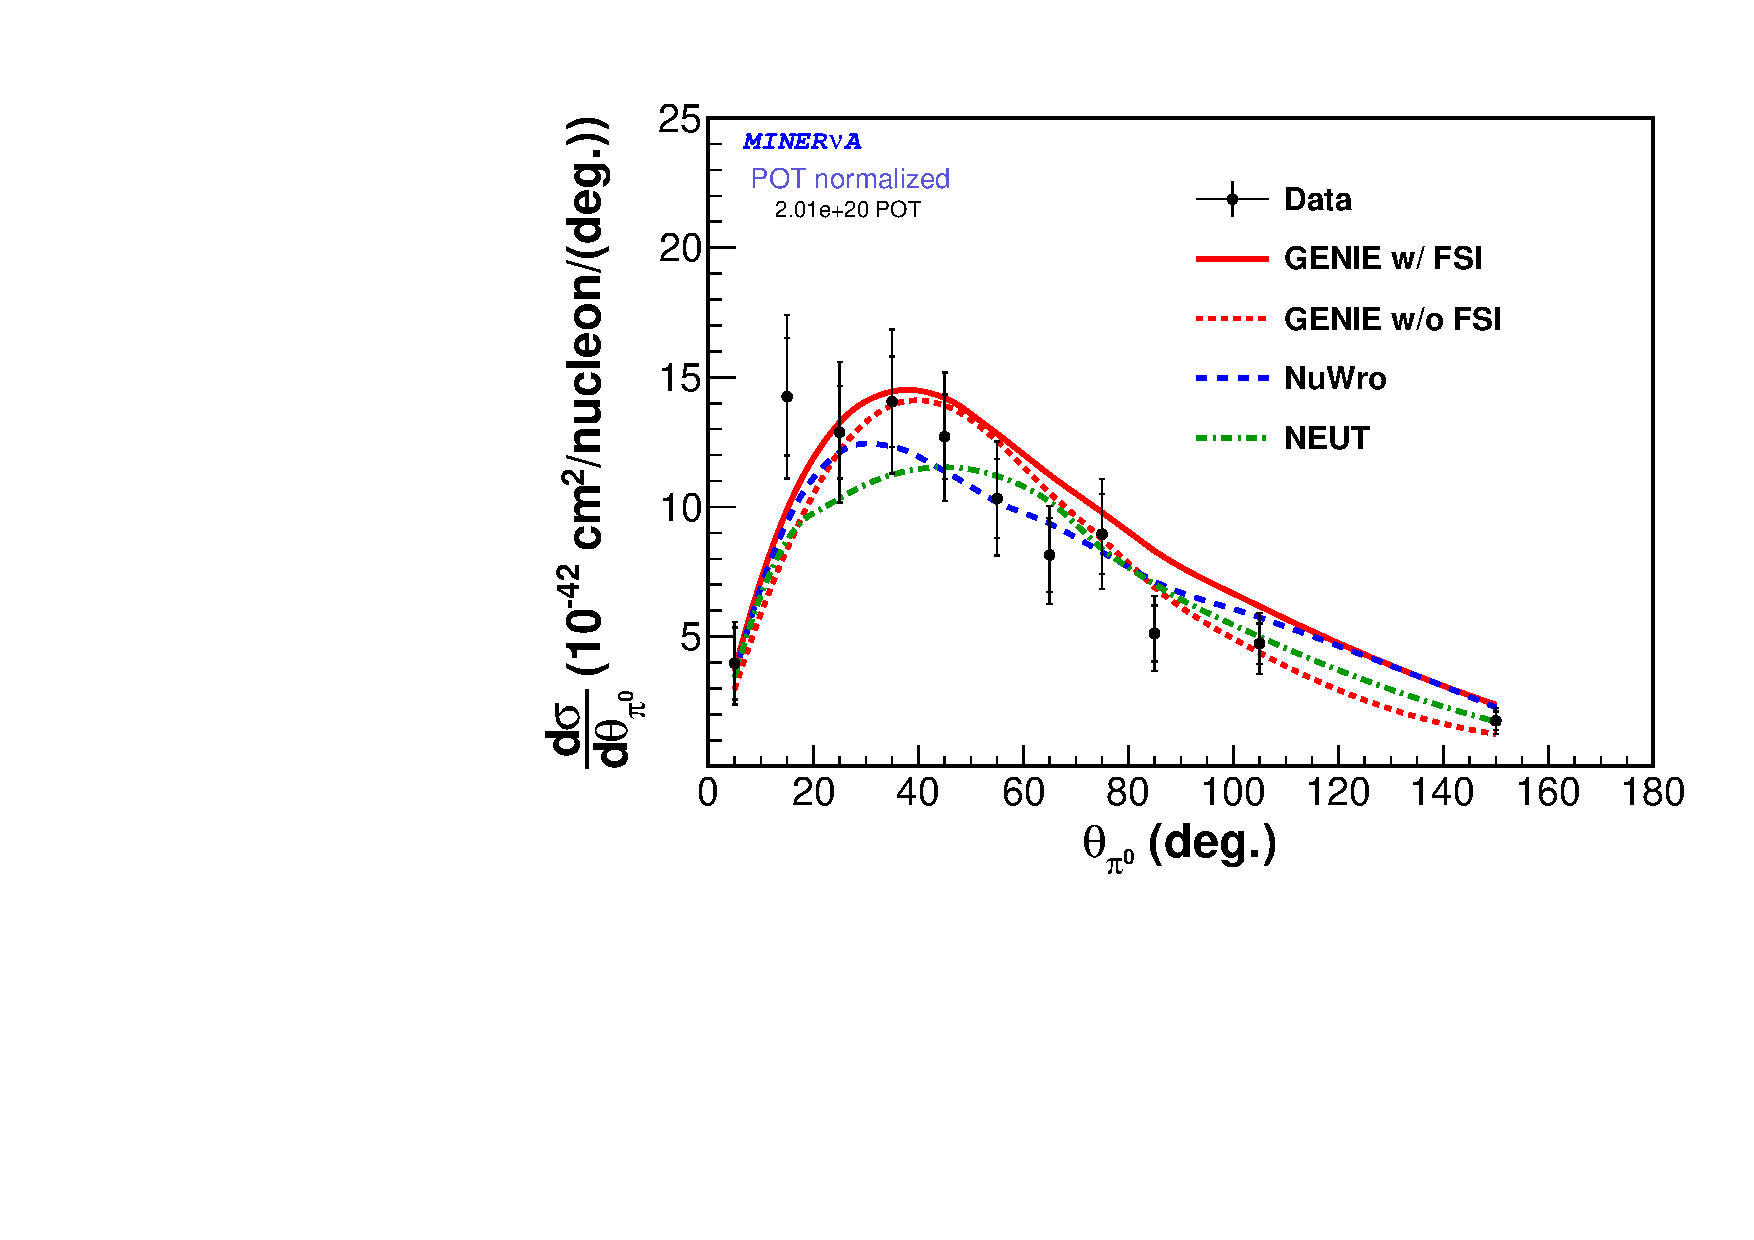
\includegraphics[width=1.0\columnwidth]{theta-data-mc-xs-multiflux-model-nuwro-pot.pdf}
\fi
    \vspace{-7pt}
\caption{Differential cross section for $1\pi^0$ production as function of the $\pi^0$ polar angle. 
Data are shown as solid circles. The inner (outer) error bars correspond to statistical (total) 
uncertainties. The solid (dashed) histograms are GENIE prediction with (without) FSI, the 
long-dashed histogram is the prediction from the NuWro generator,
and the dot-dashed histogram is the prediction from NEUT.}
\label{fig:xsec-pitheta}
\end{figure}

Figures.~\ref{fig:xsec-pimom} and \ref{fig:xsec-pitheta} also show 
predictions including FSI from the NuWro and NEUT event generators.
Any prediction requires knowledge of $\bar{\nu}_\mu N \rightarrow \mu^+ \pi^0 N$ reactions.  
Because of the dearth of data for these channels, the calculations use isospin relations 
to extrapolate from other pion production channels~\cite{Rein:1980wg,Graczyk:2009qm}. 
Both NuWro and NEUT use full cascade models~\cite{Salcedo:1987md} for the FSI description. 
The $\chi^2/$dof values for the NuWro and NEUT comparisons are 25.0/11 
and 24.9/11  for the $\pi^0$ momentum and 11.8/11 and 14.0/11 for the 
$\pi^0$ production angle, respectively. These $\chi^2$ values indicate that a 
common level of agreement is achieved by all three generators 
for $\pi^0$ momentum, and that modest differences with predictions 
versus data are observed for $\pi^0$ production angle.
%Although this approach produces good agreement for NEUT,
%predictions from NuWro and GENIE have a somewhat higher magnitude.

There are uncertainties in the FSI used in all calculations.  Each assumes the pion FSI
after production in the nuclear medium is the same as for pion beams; this assumes
no medium effects beyond Fermi momentum and a simple binding energy.  Since
$\pi^0$ beams are not possible, isospin relations must be used for $\pi^0$ FSI.
Experiments like these are valuable for testing these approximations.  In spite of
these uncertainties, the calculations give adequate descriptions of these new data.

Figures.~\ref{fig:breakdown-xsec-pimom} and \ref{fig:breakdown-xsec-pitheta} 
show decompositions of the $\pi^0$ momentum and angle spectra of
Figures.~\ref{fig:xsec-pimom} and \ref{fig:xsec-pitheta} according 
to the FSI channels as predicted by the GENIE simulation, allowing for a more detailed 
interpretation.  This shows how each FSI process changes the spectrum and gives
an indication of what refinements are needed for better agreement with data.
GENIE predicts that about 80\% of the events undergo some FSI.  In the momentum spectrum, absorption events (not shown 
in the spectrum because the pion disappears in the nucleus) 
preferentially deplete the region centered at $p_\pi \approx 0.26$ GeV/c, the momentum where the
pion-carbon total reaction cross section is a maximum~\cite{Lee:2002eq}.  On the other
hand, pion inelastic 
scattering and CEX interactions shift the pion momentum from high values to 
lower values, therefore contributing to the buildup of events at 
$p_\pi \approx 0.2$ GeV/c seen in the data.  The contributions from multi-pion production followed 
by absorption, elastic scattering, and the non-interacting
component have no noticeable effect on shape.  

For the angle spectrum FSI decomposition (Fig.~\ref{fig:breakdown-xsec-pitheta})
the effects are very different.  The interactions displayed in the figure
have a small influence on shape and the angular distribution of
the $\Delta(1232)$ decay becomes important.  The inelastic and
CEX interactions are largely responsible for the buildup of events
at backward angles.



\begin{figure}[t]
%\begin{figure}[!htpb]
\centering
\ifnum\PLsupp=0
  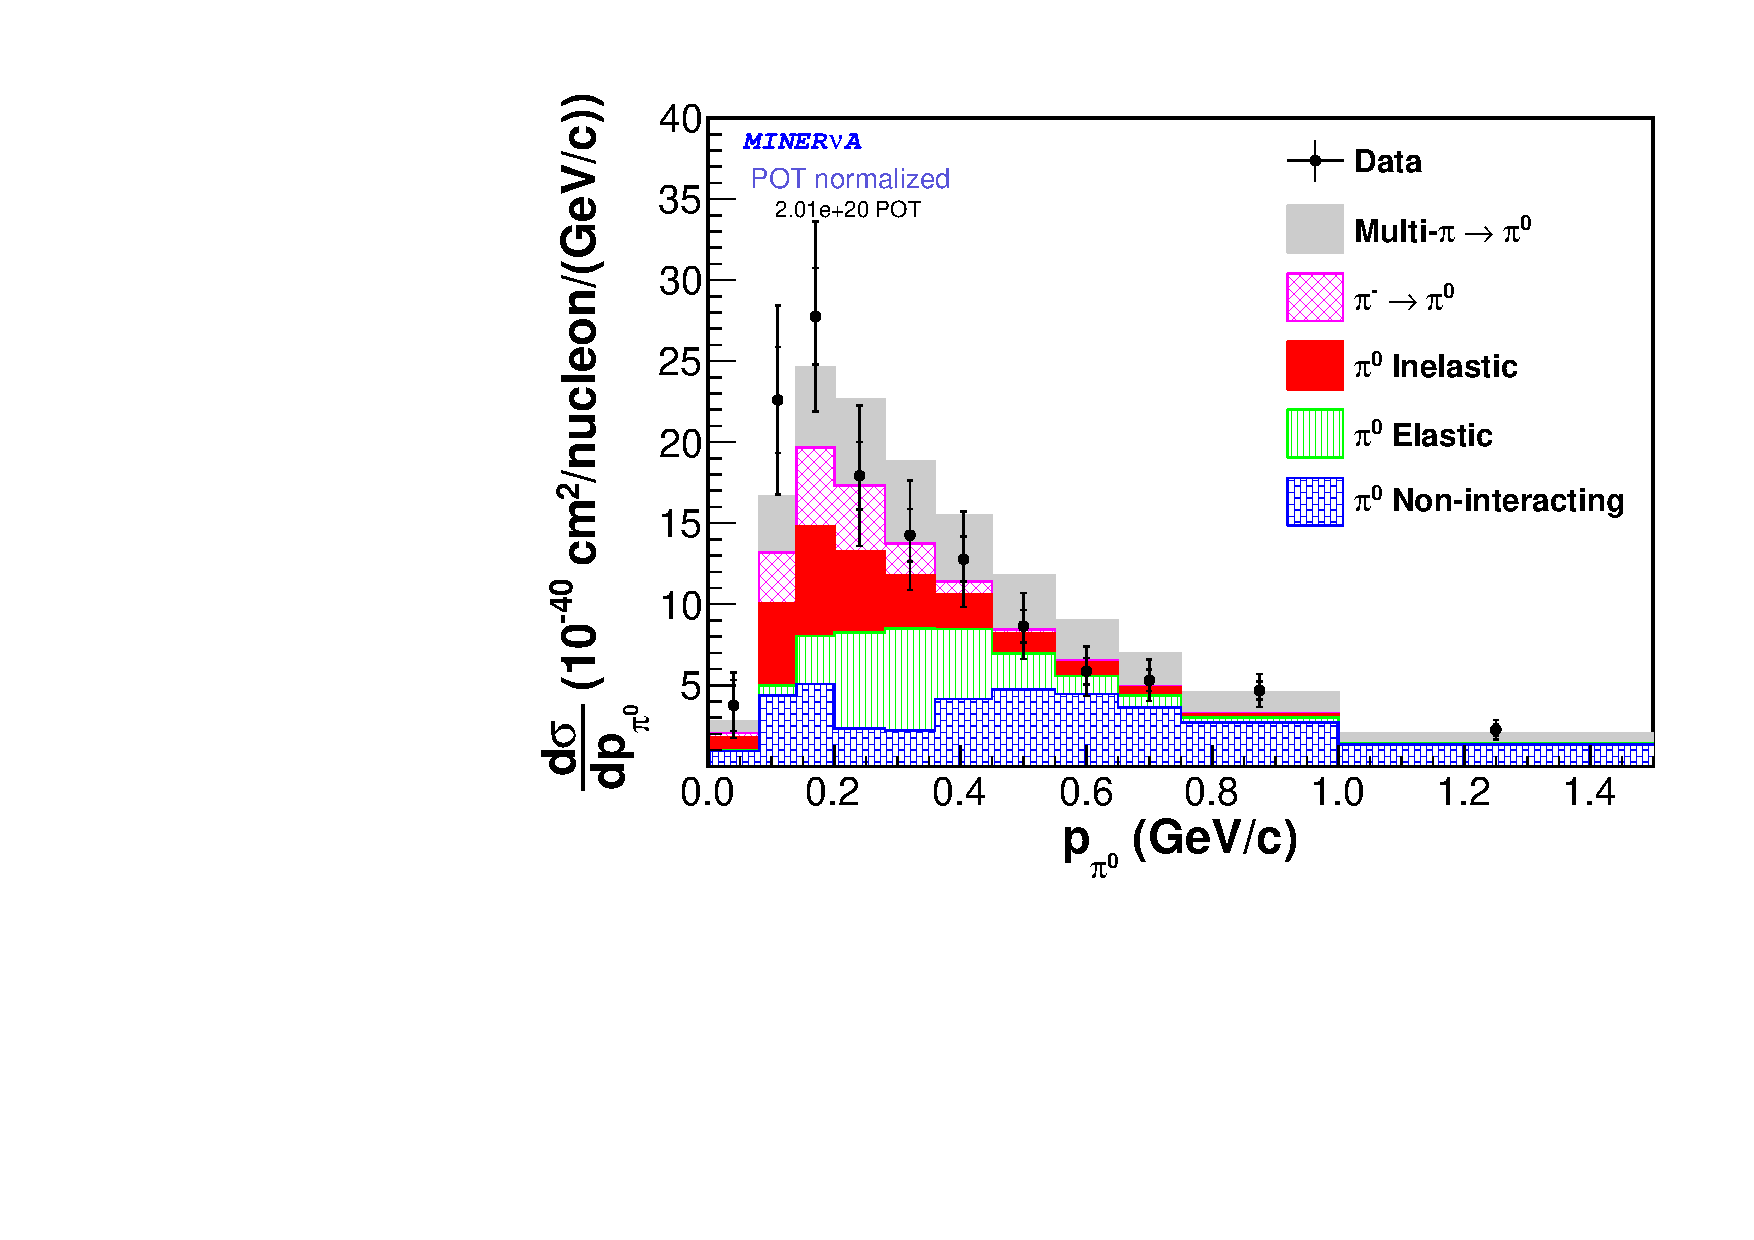
\includegraphics[width=1.0\columnwidth]{pimom-data-mc-xs-multiflux-origin-breakdown-pot.pdf}
\else
  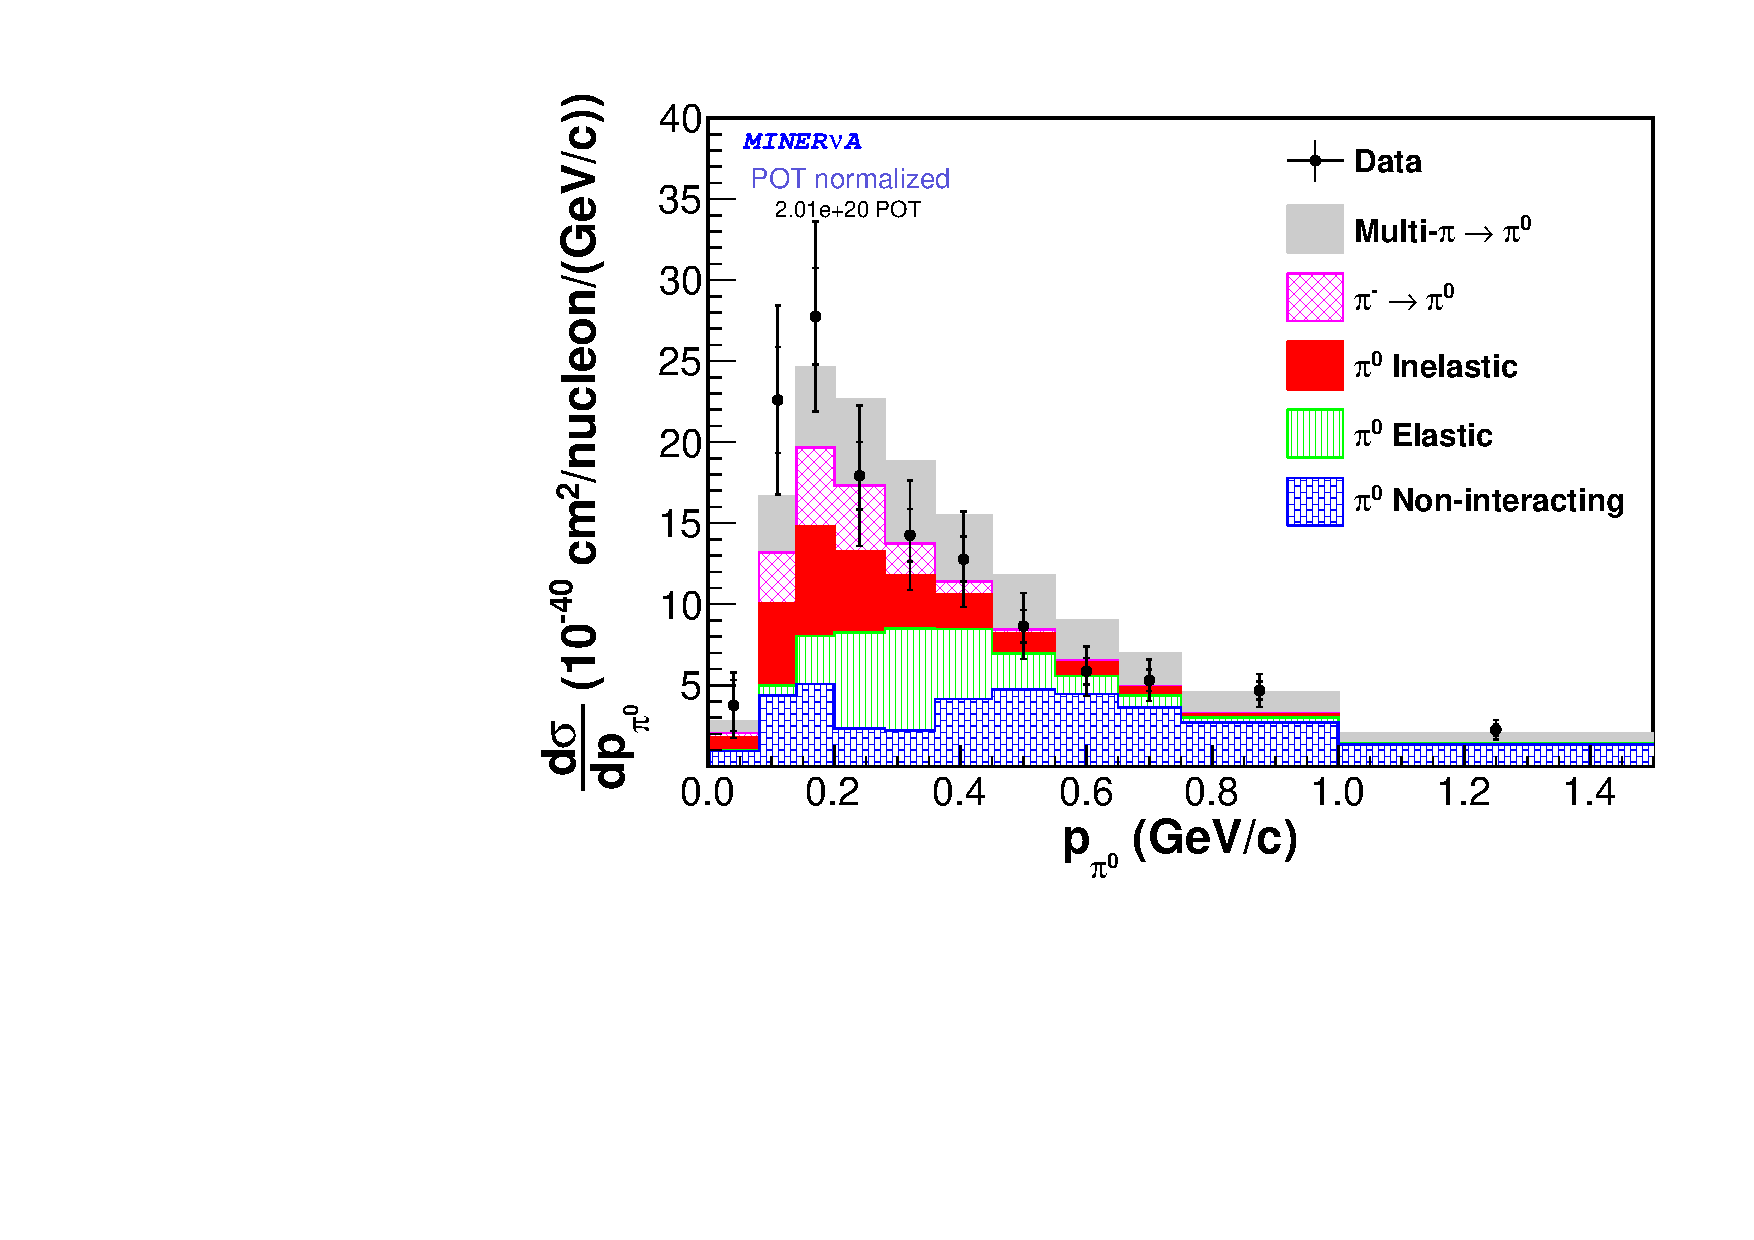
\includegraphics[width=1.0\columnwidth]{pimom-data-mc-xs-multiflux-origin-breakdown-pot.pdf}
\fi
    \vspace{-7pt}
\caption{Same cross section data as Fig. \ref{fig:xsec-pimom}.
The stacked histograms 
show a decomposition of the 1$\pi^0$ signal into different FSI channels as predicted by GENIE. 
Description of the FSI channels follows (from top to bottom):
1) Multi-$\pi\rightarrow\pi^0$: multi-pion produced by the primary interaction and all other pions are re-absorbed
inside the nucleus, except a $\pi^0$,
2) $\pi^-\rightarrow\pi^0$: a $\pi^-$ produced by the primary interaction, then charge exchanges inside the nucleus, 
3) $\pi^0$ produced by the primary interaction and then undergoing inelastic scattering inside the nucleus,
4) $\pi^0$ produced by the primary interaction and then undergoing elastic scattering inside the nucleus, and
5) $\pi^0$ produced by the primary interaction and exiting the nucleus without interacting.}
\label{fig:breakdown-xsec-pimom}
\end{figure}


\begin{figure}[t]
%\begin{figure}[!htpb]
\centering
\ifnum\PLsupp=0
  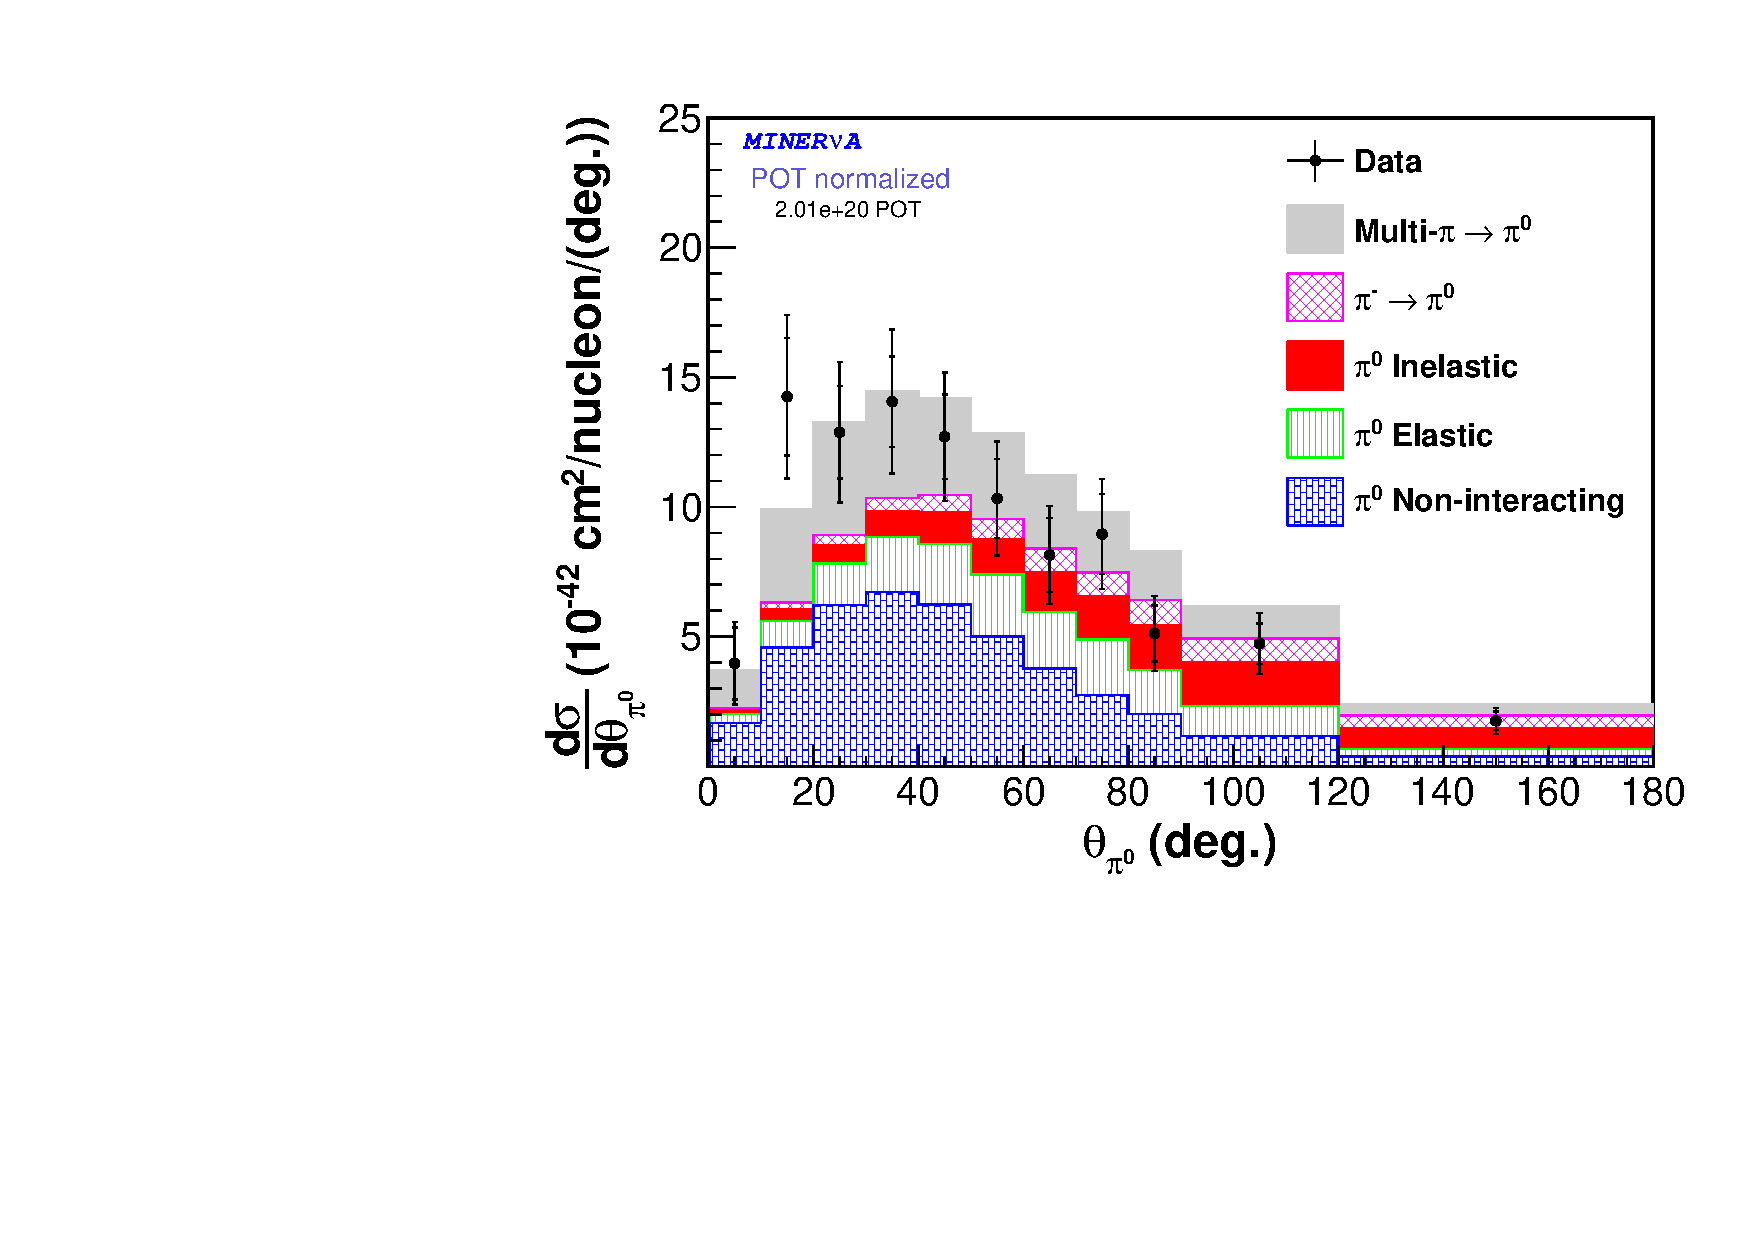
\includegraphics[width=1.0\columnwidth]{theta-data-mc-xs-multiflux-origin-breakdown-pot.pdf}
\else
  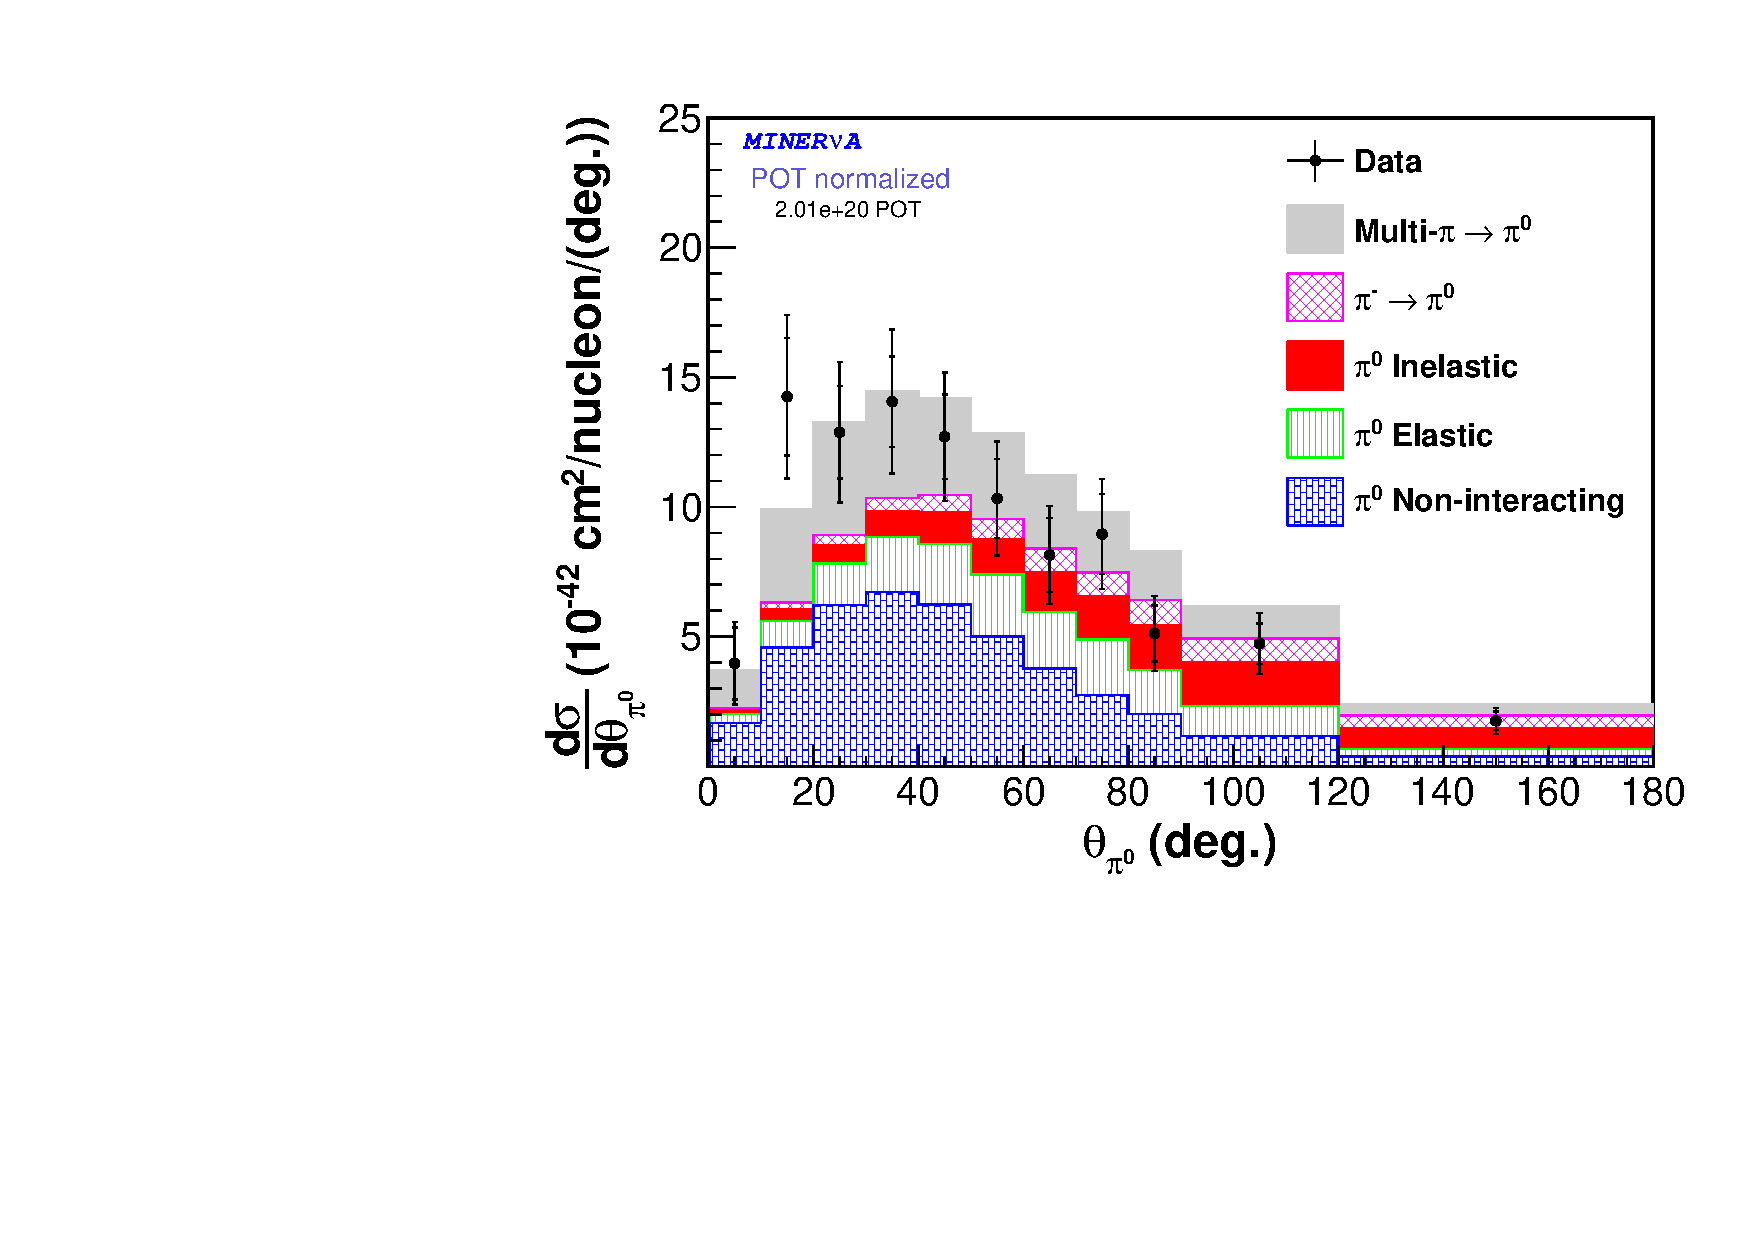
\includegraphics[width=1.0\columnwidth]{theta-data-mc-xs-multiflux-origin-breakdown-pot.pdf}
\fi
    \vspace{-7pt}
\caption{Same cross section data as Fig. \ref{fig:xsec-pitheta} and same decomposition as with Fig.~\ref{fig:breakdown-xsec-pimom}. 
The stacked histograms show a decomposition of the 1$\pi^0$ signal into different FSI channels as predicted by GENIE. 
% why repeat what is in previous figure?
%Description of the FSI channels follows (from top to bottom):
%1) $\pi^-\rightarrow\pi^0$: a $\pi^-$ produced by the primary interaction, then charge exchanges inside the nucleus, 
%2) $\pi^0+\pi\rightarrow\pi^0$: multi-pion produced by the primary interaction and all other pions are re-absorbed
%inside the nucleus, except a $\pi^0$,
%3) $\pi^0$ produced by the primary interaction and then undergoing inelastic scattering inside the nucleus,
%4) $\pi^0$ produced by the primary interaction and then undergoing elastic scattering inside the nucleus, and
%5) $\pi^0$ produced by the primary interaction and exiting the nucleus without interacting.
}
\label{fig:breakdown-xsec-pitheta}
\end{figure}

Comparison of the observed spectral shape in Fig.~\ref{fig:breakdown-xsec-pimom} to the GENIE prediction suggests
that an increase in inelastic scattering together with compensating reduction in elastic 
and/or multiple-pion production with absorption, could improve the agreement with data.
On the other hand,  Fig.~\ref{fig:breakdown-xsec-pitheta} indicates such changes would worsen the agreement with 
the data  for pion production at backwards angles.  Thus it appears that a refined 
description might require separate, independent adjustments to the two spectra.

While the previously reported information on the reaction studied here is too limited to 
enable comparisons, it is useful to compare with the recently reported MINERvA observations 
on $\nu_\mu$ induced charged pion production~\cite{Eberly:2014mra}. The latter data was obtained using a 
low-energy exposure in the same beamline, and the cross section normalizations are carried out 
in a similar way for both analyses.  Existence of both results provides stronger
constraints on the calculations. 
The $\pi^0$ momentum range in this analysis
is wider than the range shown for the charged pions of Ref.~\cite{Eberly:2014mra} (0-1.5 GeV/c versus 0.1-0.5 GeV/c) 
because the $\pi^+$ data is limited by tracking and particle identification requirements. 
Nevertheless, both analyses show that GENIE predictions are significantly improved when FSI are accounted for.   
Both results show a peak in the momentum distribution at $p_\pi \approx 0.2$ GeV/c which is seen in the GENIE calculations, 
but do not have the correct distribution at energies near this peak.
The GENIE predictions for the absolute rates for singly-produced pions exceed the observed 
rates in both analyses, however the discrepancy is less severe for production by
$\bar{\nu}_\mu$ as reported here.


\section{Conclusion}

The single differential cross sections in $\pi^0$ momentum 
and angle have been measured for 1$\pi^0$ production by $\bar{\nu}_\mu$ charged-current 
interactions in plastic scintillator (CH). 
The measurements are found to be in agreement with the predictions from 
GENIE, NuWro, and NEUT event generators. This agreement is interesting because of 
the approximations needed to make predictions
for this channel.  The measured cross section in $\pi^0$ momentum disfavors 
the GENIE prediction without FSI effects at low $\pi^0$ momentum, which is not surprising 
since FSI is expected for hadrons inside nuclei. A decomposition 
of the FSI effects shows that inelastic scattering and CEX reactions
are responsible for the peak at $p_\pi\approx 0.2$ GeV/c. These contributions
could be adjusted within external experimental errors to achieve
even better agreement of calculations with the $\pi^0$ momentum data.
However, these changes would not be as effective for the $\pi^0$ polar angle. 

Charged-current single pion production in the few GeV region of neutrino energy is an important 
class of interactions in long-baseline neutrino oscillation experiments.   This work presents 
the first detailed measurements of the kinematic distributions for single $\pi^0$s produced 
in charged current $\bar{\nu}_\mu$ interactions on carbon.  These distributions provide 
constraints on antineutrino-induced $\pi^0$ backgrounds as will occur in $\bar{\nu}_e$ appearance 
experiments.  

